\section{Algorithm Explanation}

The final version here presented is a software that can be divided in the following parts: Hand Segmentation, Hand Description and Gesture Interface.

\subsection{Hand Segmentation}
The segmentation of the hand was one of the most important parts of the software since in it depends the correct functioning of the next parts. 
The flowchart of this part of the code is as follows: 

\begin{figure}[H]
	\centering
	 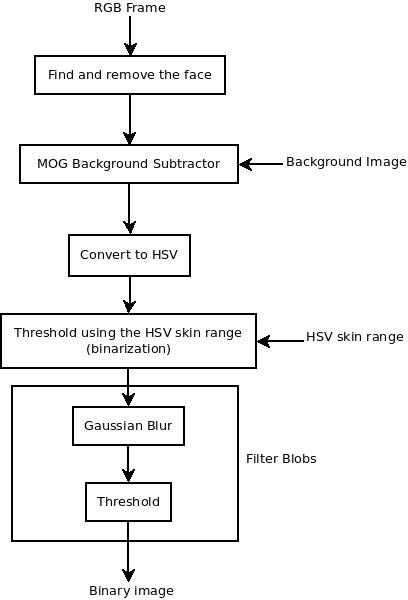
\includegraphics[width=0.4\textwidth]{../hand_filter.jpeg} 
\end{figure}
 
As it can be seen in the diagram, the first thing done is to detect the face using the "Face Detection using Haar Cascades" already implemented and trained in OpenCV. It is a very reliable clasifier because of the huge dataset used in the training phase. It was used this one instead of making our own in order to have a reliable detector without spending too much time on it, as is just a small part of the segmentation. 


After the face detection, a binary mask is made in which a black square is drawn over the face to hide it.

Next, a Mixture of Gaussians background subtractor is used to remove the background of the image and detect more easily the hand. From this step, another binary mask is created and applied to the original image. 
The background subtractor is inherited from the class cv::BackgroundSubtractorMOG2 made in order to modify the protected parameter "backgroundRatio". This parameter measures the frequency at which the background image is updated. In this code, the backgroundRatio is a very low number to make the background update as low as possible. This allows the user to keep the hand in the same position for a while without being recognized as background.  

Afterwards, the resulting image with the latter masks being applied is converted to the HSV color space and is thresholded using the appropriate HSV skin range.
This skin range can be modified at the begining of the program, selecting the theoretical range or calculating a custom range from a skin color sample. Also, is is possible to manually adjust the minimum and maximum HSV values in another window before starting the gesture recognition. 

Finally, in order to better the output binary image, a gaussian blur and a thresholding is applied to eliminate blobs and unite different regions of the hand. It was chosen this configuration because it was much faster and gave better results than making an opening to the image. 

 
\subsection{Hand Description}

The input of this section is the binary image that was the output of the previous one. This part of the software characterizes and extracts the hand parameters. 

\begin{figure}[H]
	\centering
	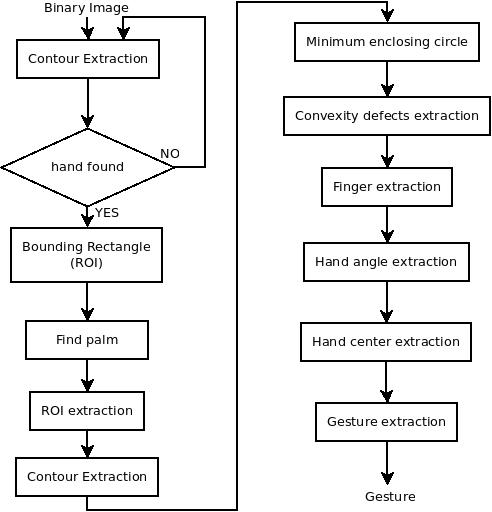
\includegraphics[width=0.5\textwidth]{../hand_description.jpeg} 
\end{figure}


The first step is to find all the contours on the binary image, and discard the ones that are too small, as they are likely noise blobs on the image. Once the small contours are filtered, a polygon approximation is carried out to make the contour smaller and reduce the computational load of the algorithm.

If a contour large enough is found, it calculates the bounding box of the contour and the minimum rotated rectangle bounding the contour, for the later angle calculation. Then, the maximum inscribed circunference, that describes the hand palm, is found by calculating the point which maximizes the distance to the hand contour (the inscribed circle center), and its distance (the inscribed circle radius).

The hand is supposed to be inside a circunference of 3.5 times the radius of the maximum inscribed circunference, so we extract that region of interest and find the contours again inside that region, to eliminate any contour due to the forearm skin. The minimum enclosing circunference for that contour is found, which will be used for closed fist / open palm gesture detection.

For the finger detection, the first step is to calculate the convex hull of the hand contour, and then find the convexity defects, the points of the original contour between the vertex of the convex hull that are the furthest away from the hull segment. Each of that defects will represent the valley between two potential fingers, but before they can be considered fingers they have to fulfill three conditions:

\begin{enumerate}
\item The depth of the convexity defect must be in between the minimum bounding circunference radius and the maximum inscribed circunference radius. 
\item The angle between the segments joining the defect depth point and the defect start/end points that represents the angle between two consecutive fingers, must be lower than 90º.
\item The last condition is related to the k-curvature, that should be lower than 70º. The k-curvature is the angle between two segments joining a point close to the fingertip and a point of the contour k places before and after that point. For our software, the value of k chosen was 9, but if the contours used had more points one should increase this value. This condition allows us to find the fingerprint points more accurately.
\end{enumerate}

Those points that fulfilled these three conditions and that were close enough were considered as the same fingerprint.

This method works very well with most of the gestures except for the case when the hand has only one finger shown, as the resultant contour will not have any hull defect that accomplishes these conditions.

Next, the angle and center of the hand are extracted and filtered using a Kalman filter, for smoothing the output values and getting a more constant cursor trajectory that allows the user to select buttons and GUI controls more precisely.

Finally, the gesture of the hand is guessed based on the hand descriptors previously extracted. The gestures implemented in this version are:

\begin{itemize}
\item {\bfseries Open palm:} number of fingers found is either 4 or 5.
\item {\bfseries Closed fist:} no fingers were detected, the ratio between the minimum enclosing circunference radius and the maximum inscribed circunference radius is less than 2.
\item {\bfseries Victory sign:} two fingers found, angle between them less than 60º.
\item {\bfseries Gun sign:} two fingers found, angle between them more than 60º (and less than 90º).
\item {\bfseries No gesture found:} The descriptors extracted do not match any of the previous conditions.
\end{itemize}

Those gestures are encoded using a integer value and used by other parts of the software.


\subsection{Gesture Interface} 

The gesture interface takes as input the gesture guess data from the previous hand description stage, and triggers several actions depending on the gesture and the configuration selected. Due to the presence of false positives and false negatives in the output of the previous stage, and as it could trigger unwanted actions on the computer, a simple state machine is implemented to assure that the program triggers these actions only when they are desired by the user.

The state machine has two states, ``found'' and ``not found'', representing the cases in which the gesture has ocurred or it has not ocurred yet, respectively. It also has two counters, one counting the number of positive matches with the value to track, and the other the number of consecutive negative matches.

If the number of consecutive negative matches is equal to the maximum value allowed, it resets the positive matches counter. If the the number of positive matches equals the minimum value of positive matches needed, it reaches the ``found'' state, and stays there until it is reseted (either by the user or by the arrival of negative matches). 


This interface allows the user to control the cursor and move it around when a ``open hand'' gesture is detected, and to click with a ``closed fist'' gesture. It also allows to launch two different commands with the remaining implemented gestures, than can be configured with a configuration file.

More information about the configuration file, the gestures and how to use the software in the ``User Guide''. 

\newpage